%\documentclass[utf8]{FrontiersinHarvard} % for articles in journals using the Harvard Referencing Style (Author-Date), for Frontiers Reference Styles by Journal: https://zendesk.frontiersin.org/hc/en-us/articles/360017860337-Frontiers-Reference-Styles-by-Journal
%\documentclass[utf8]{FrontiersinVancouver} % for articles in journals using the Vancouver Reference Style (Numbered), for Frontiers Reference Styles by Journal: https://zendesk.frontiersin.org/hc/en-us/articles/360017860337-Frontiers-Reference-Styles-by-Journal
\documentclass[utf8]{frontiersinFPHY_FAMS} % Vancouver Reference Style (Numbered) for articles in the journals "Frontiers in Physics" and "Frontiers in Applied Mathematics and Statistics" 

%\setcitestyle{square} % for articles in the journals "Frontiers in Physics" and "Frontiers in Applied Mathematics and Statistics" 
\usepackage{url,hyperref,lineno,microtype,subcaption}
\usepackage[onehalfspacing]{setspace}
\raggedbottom
\linenumbers


% Leave a blank line between paragraphs instead of using \\


\def\keyFont{\fontsize{8}{11}\helveticabold }
\def\firstAuthorLast{Olp {et~al.}} %use et al only if is more than 1 author
\def\Authors{Michael D. Olp\,$^{1, *}$, Vincent A. Laufer\,$^{1}$,  Andrew L. Velesano\,$^{1, 2}$, Andrea Zimmerman\,$^{1}$, Kenneth J. Woodside\,$^{3, 4, 5}$, Yee Lu\,$^{6}$, Adam S. Lauring \,$^{2}$, and Matthew F. Cusick\,$^{1,*}$}
% Affiliations should be keyed to the author's name with superscript numbers and be listed as follows: Laboratory, Institute, Department, Organization, City, State abbreviation (USA, Canada, Australia), and Country (without detailed address information such as city zip codes or street names).
% If one of the authors has a change of address, list the new address below the correspondence details using a superscript symbol and use the same symbol to indicate the author in the author list.
\def\Address{$^{1}$Department of Pathology, University of Michigan, Ann Arbor, MI, USA \\
$^{2}$Division of Infectious Diseases, Department of Internal Medicine and Department\\ of Microbiology and Immunology, University of Michigan, Ann Arbor, MI, USA\\
$^{3}$Sharing Hope of South Carolina, Charleston, SC, USA\\
$^{4}$Gift of Life Michigan, Ann Arbor, MI, USA\\
$^{5}$Academia Invisus LLC, Ann Arbor, MI, USA\\
$^{6}$Division of Nephrology, Department of Internal Medicine, University of Michigan, Ann Arbor, MI, USA}
% The Corresponding Author should be marked with an asterisk
% Provide the exact contact address (this time including street name and city zip code) and email of the corresponding author
\def\corrAuthor{2800 Plymouth Rd building 35, Ann Arbor, MI 48109}

\def\corrEmail{olpmi@med.umich.edu, mfcusick@med.umich.edu}




\begin{document}
\onecolumn
\firstpage{1}

\title {HLA-C Peptide Repertoires as Predictors of Clinical Response During Early SARS-CoV-2 Infection} 

\author[\firstAuthorLast ]{\Authors} %This field will be automatically populated
\address{} %This field will be automatically populated
\correspondance{} %This field will be automatically populated

\extraAuth{}% If there are more than 1 corresponding author, comment this line and uncomment the next one.
%\extraAuth{corresponding Author2 \\ Laboratory X2, Institute X2, Department X2, Organization X2, Street X2, City X2 , State XX2 (only USA, Canada and Australia), Zip Code2, X2 Country X2, email2@uni2.edu}


\maketitle


\begin{abstract}

The Human Leukocyte Antigen (HLA) system plays a pivotal role in the immune response to viral infections, mediating the presentation of viral peptides to T cells and thereby influencing both the strength and specificity of the host immune response. Variations in HLA genotypes across individuals can lead to significant differences in susceptibility to infections and the severity of disease outcomes. This study leverages insights from the early phase of the COVID-19 pandemic to explore how specific HLA class I molecules, particularly HLA-C, affect the clinical response to SARS-CoV-2 infection. By analyzing high-resolution HLA typing and viral genomic sequences from 60 patients, we assess the correlation between HLA-C peptide binding repertoires and disease severity, as measured by the Sequential Organ Failure Assessment (SOFA) score. Our findings reveal a significant link between the extent of viral peptide binding by HLA-C molecules and infection outcomes, with broader HLA-C peptide binding repertoires associated with more severe disease manifestations. Furthermore, the study delves into the impact of viral sequence variation on HLA-C-mediated immune responses, underscoring the critical role of HLA-C in shaping the host's defense mechanisms against SARS-CoV-2. These results highlight the importance of considering HLA diversity in developing vaccines and managing viral infections, providing valuable lessons for understanding host-pathogen interactions and advancing personalized medicine approaches in combating viral diseases. 

\tiny
 \keyFont{ \section{Keywords:} HLA, SARS-CoV-2, antigenicity, bioinformatics, computational biology}
\end{abstract}

\section{Introduction}

Symptoms of infection by severe acute respiratory syndrome coronavirus type 2 (SARS-CoV-2) range from mild common cold-like symptoms to severe pneumonia, including progression to acute respiratory distress syndrome (ARDS) and multisystem organ failure (MOF) \citep{32064853, 32134116}. While demographic, medical, and behavioral risk factors influence outcomes \citep{32335169}, dysregulated activation of immune responses is also implicated in severe clinical progression early in infection \citep{31986264, 32085846}. Imbalances of the immune system result in pathological inflammatory responses. Host genetic responses to exogenous pathogens can result in an inadequate response with the host succumbing to the infection, an adequate response with containment of the infection, or an excessive response resulting in host tissue damage. 

Human leukocyte antigen (HLA) genes are highly polymorphic structures with central roles in shaping immune responses against pathogens. The interactions between HLA I and II molecules and T cell receptors (TCR) activate lymphocytes and develop the adaptive immune effector milieu. HLA class I antigens interact with cytotoxic T cells (CD8+) and kill virally infected targets. HLA class II antigens are involved in presenting exogenous antigens to T helper (CD4+) cells for coordinating immunospecific responses. Different HLA genes determine specific repertoires of peptides included in the major histocompatibility complex (MHC) and influence subsequent TCR recognition, leading to antigen-specific immune responses. Therefore, HLA heterogeneity is a crucial factor underlying differential susceptibility to viral infection across human populations.  

Specific HLA alleles and haplotypes impact severity and progression of viral infection due to Human Immunodeficiency virus (HIV) \citep{22999948, 10073943, 12352262, 21051598}, hepatitis B \citep{27243039, 24842861}, hepatitis C \citep{16571411, 16343061, 18074415}, and influenza \citep{19234171, 11836437, 29315655}. Certain HLA alleles have also been associated with poor clinical response to infection by SARS-CoV \citep{12969506, 32297958}, a closely related predecessor to SARS-CoV-2 with approximately 80\% genetic sequence identity \citep{32027036, 32007145}. However, geographic restriction of SARS-CoV transmission allowed for examination of only limited pools of HLA alleles. In contrast, the pandemic nature of SARS-CoV-2 has prompted numerous studies analyzing broader ranges of HLA alleles. These efforts have identified multiple associations between patient HLA alleles and disease outcome \citep{34490415, 33968060, 33734601, 33298875, 33896121, 34294460, 35960731, 37468623, 37112884, 36627290, 36534127}. However,  identified associations are not entirely consistent \cite{36534127, 38251811}. Discrepancies in allele-level associations between studies are at least partially due to geographic variation in HLA genotype frequency. In addition, geographic and temporal SARS-CoV-2 genetic variation further complicates comparison across studies.  

SARS-CoV-2 mutational analysis has been a crucial component of vaccine design, and HLA has emerged as an important target \citep{32106567, 32269766, 32303592, 32295479, 35577837}. \textit{In silico} peptide binding analyses have been instrumental in identifying antigenic SARS-CoV-2 peptides given the particularly large viral peptidome as well as the combinatorial nature of binding groove sequence variation both within and across HLA loci. Machine learning tools like NetMHCpan and NetMHCIIpan utilize available experimental data to allow robust and efficient prediction of MHC-peptide binding \citep{32406916}. While high-affinity MHC-peptide binding does not, by itself, equate with immunogenicity, in silico techniques have successfully identified SARS-CoV-2 epitopes capable of eliciting T cell response, many of which are HLA specific \citep{33128877, 33853928, 33184509}. Importantly, even sequence variation within SARS-CoV-2 lineages may alter the presentation of viral peptides by HLA molecules \citep{34396391}. 

Here, we employ \textit{in silico} peptide binding prediction to investigate the role of individual HLA classification in clinical response to SARS-CoV-2 infection. Individual levels of viral peptide binding to class I and II HLA molecules were predicted using paired six-locus high-resolution HLA typing and SARS-CoV-2 genomic sequencing for 60 patients presenting to Michigan Medicine within 10 days of a positive PCR test. We then test the hypothesis that variation in viral antigenicity is associated with differential clinical response to infection using the Sequential Organ Failure Assessment (SOFA) scoring system as an indicator of disease severity. This is the first study comparing HLA classification with clinical outcome that controls for SARS-CoV-2 genomic sequence variation at an individual level. Using a multiple linear regression-based approach that accounts for six-locus HLA genotype and demographic factors, we identify a significant association between unbalanced HLA-C-mediated peptide binding and severe disease following SARS-CoV-2 infection. Molecular modeling and unsupervised machine learning techniques provide structural and functional insight into differential peptide binding by individual HLA-C molecules that correlate with disease severity. In addition, we investigate how viral sequence variation over time affects disproportionate HLA-C-mediated peptide binding. Ultimately, this research aims to enhance understanding of how individual HLA classification impacts interaction with novel antigens to influence clinical outcomes, both in the context of continuing SARS-CoV-2 transmission and novel viral pathogens.

\section{Results}
\subsection*{Extent of patient HLA-C peptide binding repertoire is a risk factor for severe SARS-CoV-2 infection.} In order to investigate relationships between HLA class I genotype and illness severity following SARS-CoV-2 infection, high-resolution HLA types and viral genomic sequences were obtained for 60 patients with positive polymerase chain reaction (PCR) tests between March 24, 2020, and May 5, 2020.  This study design allows direct comparison between each patient’s HLA class I alleles and the specific peptidome encoded by their SARS-CoV-2 strain. Infection severity is quantified as the maximum sequential organ failure assessment (SOFA) score documented within 10 days of SARS-CoV-2 diagnosis. Here, SOFA score shows a significant positive correlation with laboratory values previously associated with severe disease, including creatinine, white blood cell count (WBC), and C-reactive protein (CRP) \citep{32533986, 32533986}, as well as indications of poor outcome such as intensive care unit (ICU) admission and need for intubation (Figure S1).

To allow associations between the extent of viral peptide recognition by patient-encoded MHC class I molecules and clinical outcome following SARS-CoV-2 infection, binding predictions were performed using NetMHCpan software. Binding affinity (BA) and mass spectrometry-based eluted ligand (EL) scores were calculated for all MHCI:peptide pairs resulting from each patient’s six HLA class I alleles and the corresponding SARS-CoV-2 peptidome, including sequences eight to eleven amino acids in length (Figure 1A-C, Table S2-4). In addition, MHCI:peptide pairs were queried in the Immune Epitope Database (IEDB) to identify experimentally validated binding interactions as well as pairs showing no binding. The resulting 2,431 experimentally interrogated MHCI:peptide pairs were used as a training set for logistic regression to assign binding probabilities for all NetMHCpan predictions (Figure 1E). The overall logistic regression model is closely related to the binding affinity score (Figure 1D).

To test the hypothesis that response to infection is related to the overall size of patient HLA class I peptide binding repertoires, the sum of predicted interactions for each patient’s two HLA-A, -B, and -C alleles were used to predict SOFA score in bayesian generalized linear multivariate regression (Figure 1F, S2). To avoid spurious results due to ambiguity regarding biologically relevant MHC:peptide binding affinities and the use of a single arbitrary cutoff to define binding, numbers of peptide interactions were calculated over a range of probability cutoffs (0.5 – 0.9) (Figure D-F). The resulting distributions were then accounted for as independent variable uncertainty using Bayesian techniques \citep{RJ-2018-017, Carpenter2017}. In addition, age, body mass index (BMI), and sex were included as regressors to control for potential influences of these demographic factors over the clinical course. Of the variables examined, increased size of HLA-C peptide binding repertoire predicts poor response to infection as the corresponding 95\% confidence interval does not include zero (Figure 1F). Although not reaching statistical significance, increased SOFA score was predicted by decreased sizes of HLA-A and -B peptide binding repertoires. Together, these results predict disproportionate peptide binding by HLA-C molecules relative to HLA-A and -B is a risk factor for severe SARS-CoV-2 infection.

\subsection*{Disproportionate HLA-C binding of structural and nonstructural protein sequences contributes to poor prognosis.} Early efforts aimed at epitope mapping and vaccine design primarily focused on SARS-CoV-2 structural proteins, particularly Spike. However, peptides derived from nonstructural and accessory proteins can also elicit an immune response to SARS-CoV-2 infection \citep{32473127, 32887977}. As a result, HLA class I binding was examined toward sequences derived from all twenty-seven SARS-CoV-2-encoded proteins (Figure 2A). To identify protein sequences leading to unbalanced HLA-C peptide binding relative to HLA-A and -B, predicted repertoire sizes for individual SARS-CoV-2 proteins were compared with the SOFA score for each patient. HLA class I peptide repertoire sizes for each SARS-CoV-2 protein were calculated across binding probability thresholds 0.5 to 0.9. Significant relationships with SOFA score were then identified as those with Pearson correlation coefficients with a magnitude greater than one standard deviation above 0.25, corresponding to p$<$0.05 for sixty samples.  In this analysis, quantities of predicted HLA-C peptide-binding interactions show a significant positive correlation with SOFA score for twenty of the twenty-seven SARS-CoV-2 proteins (Figure 2B). Conversely, peptide repertoire sizes for HLA-A and -B are predominantly lower for patients with more severe infection, although these correlations for individual protein sequences do not reach statistical significance. These results indicate that the disproportionate binding of HLA-C molecules toward peptides derived from structural, nonstructural, and accessory SARS-CoV-2 protein sequences contributes to an elevated risk of severe infection.

 Peptide sequence characteristics associated with differential HLA-C binding in mild versus severe SARS-CoV-2 infection were also examined. Pearson correlations were calculated between HLA-C binding probability and SOFA score for all peptides, and the top 1\% of positively and negatively correlated sequences were compared. Peptide sequences predicted to preferentially bind to HLA-C alleles encoded by patients with severe SARS-CoV-2 infection primarily show amino-acid restriction at the second from N-terminal (P2) and C-terminal anchor positions (Figure 2C-F). The C-terminal position is enriched for hydrophobic residues, which is consistent with HLA-C binding specificity overall \citep{25311805}. P2 also shows enrichment for hydroxyl-containing amino acids (Ser, Thr, and Tyr) or the smaller Ala in peptides selectively binding HLA-C alleles encoded by patients with severe infection (Figure 2C-F). While all SARS-CoV-2 sequences identified in this study are of either the A or B.1 lineages (Table S1), amino acid differences exist at sixty-two missense mutation sites. Five of these mutations significantly altered distributions of binding probability scores across patient HLA-C alleles (Figure 2G). Mutations of non-structural protein 3 (NSP3) and nucleocapsid protein (N) affect the P2 anchor, with Ser being favored for HLA-C binding. Mutations involving the C-terminal anchor of peptides derived from NSP13 and the NS3 accessory protein highlight preference for Val at this position. In addition, the Spike D614G mutation that has been associated with enhanced viral fitness is predicted to result in less HLA-C binding in this patient cohort (Figure 2G). These results implicate structural, nonstructural, and accessory protein sequences in differential HLA-C peptide binding and prognostic impact. Furthermore, missense mutations within single SARS-CoV-2 lineages can alter recognition by HLA-C molecules due to amino acid changes at the P2 and C-terminal anchor positions.
 
\subsection*{Infection severity correlates with increasing overlap between HLA-A and -C peptide binding repertoires.} Unbalanced viral peptide binding by HLA-C relative to HLA-A and -B during infection may be exacerbated by competition for shared ligands. Indeed, distributions of peptide binding across SARS-CoV-2 proteins are similar for each of the three HLA class I loci (Figure 2A). To test this hypothesis, intersections between sets of SARS-CoV-2 peptides recognized by patient HLA-A, -B, and -C alleles were determined over a range of prediction scoring thresholds (Figure 3A-B). For all patient alleles combined, percentages of HLA-A and -B peptide repertoires that are also predicted to be bound by HLA-C alleles range from 10 - 29\% and 16 – 36\%, respectively. In general, the highest degree of overlap is seen for interactions with lower predicted affinity (Figure 1D-E, 3A-B). The intersection between HLA-A and -C peptide repertoires is significantly correlated with SOFA score (Figure 3C, p $<$ 0.004). However, no similar relationship between HLA-B and -C peptide repertoires is identified (Figure 3D). These results suggest that competition between HLA-A and -C for shared SARS-CoV-2 epitopes contributes to inefficient HLA class I responses that predispose patients toward severe infection. 

\subsection*{Prognosis is not related to KIR ligand group for patient alleles.} HLA-C molecules are the primary ligands of Killer cell immunoglobulin-like receptors (KIRs), thus playing an important role in natural killer (NK) cell-mediated responses to infection \citep{11861603, 18650461}. A balanced dimorphism at amino acids 77 and 80 divides HLA-C molecules into C1 and C2 KIR ligand groups \citep{8265660} (Figure 4A-B).  C1 allotypes have previously been predicted to bind larger quantities of SARS-CoV-2 peptides \citep{32810602}, and several have been individually identified as risk factors for poor prognosis \citep{32988645, 32717807, 32717807, 35960731, 34490415, 33343579, 34289534, 34722002, 33298875, 32988645}. In the present study, C1 allotypes are also predicted to bind larger numbers of SARS-CoV-2 peptides compared with C2 allotypes (p $<$ 0.002, Figure 4C). However, comparing patient SOFA score with each of their two HLA-C alleles does not show a significant difference in prognosis between KIR ligand groups (Figure 4D, p $>$ 0.98). These results argue against KIR ligand specificity as a primary mechanism of prognostic variation in this patient cohort.

\subsection*{HLA-C peptide binding site amino acid sequence predicts patient prognosis following SARS-CoV-2 infection.} The balanced dimorphism defining KIR ligand groups has only a limited impact on the HLA-C peptide binding surface (Figure 4A). Alleles were clustered based on their complete peptide binding site amino acid sequences to examine the relationship between HLA-C molecular structure and differences in patient prognosis (Figure 5A). Distinct electrostatic patterns are qualitatively seen between the resulting groups where Cluster 1 and 2 peptide binding grooves are predominantly negatively and positively charged, respectively, whereas Cluster 3 binding sites are relatively hydrophobic (Figure 5B-D). Comparing patient SOFA scores with each of their two HLA-C alleles reveals differential prognosis across sequence-based clusters (Figure 5E, ANOVA p = 0.05). Again, severe SARS-CoV-2 infection is associated with larger HLA-C peptide binding repertoires (Figure 5F, ANOVA p $<$ 1e-11). Cluster 3 alleles are predicted to have the largest peptide binding repertoire and are associated with the greatest prognostic risk. Lower peptide binding selectivity in Cluster 3 may be due to the ability of relatively hydrophobic binding pockets to accommodate peptides with uncharged residues at P2 (Figure 2C and 5G). In addition, Clusters 1 and 3, the lowest and highest risk sequence-based groups, respectively, show allele dosage effect approaching statistical significance (p = 0.15 and 0.12, respectively; Figure S3). These results support a mechanism by which HLA-C molecule amino-acid composition and differential peptide binding specificity impact patient response to SARS-CoV-2 infection.

\section*{Discussion}

The high degree of polymorphism in the HLA system makes it an attractive target for investigations aimed at understanding genetic causes of differential responses to infection across human populations. HLA class I molecules are crucial for early elimination of virus-infected cells by CD8+ T-cells and NK cells while also maintaining self-tolerance to avoid excessive tissue damage. As a result, HLA class I genotype has received significant attention with respect to unbalanced immune responses during early SARS-CoV-2 infection. Here, we compared HLA class I genotypes and strain-specific SARS-CoV-2 peptidomes for 60 patients seen at Michigan Medicine early in the COVID-19 pandemic to investigate relationships between predicted peptide recognition and infection severity. This analysis shows patients with larger quantities of HLA-C:viral peptide interactions were significantly more likely to experience severe symptoms (Figure 1F). 

HLA-C molecules are expressed in lower quantities at the cell surface \citep{332508, 1383381, 332508, 2967765, 7760000}, compared with HLA-A and -B and, therefore, often receive less attention in studies of responses to viral infection.   Nevertheless, HLA-C-restricted viral peptides have been implicated during disease progression in HIV \citep{21814282, 22807681, 26575988, 24785948, 27880898, 32501836}, and hepatitis C infections \citep{27057987}. While the role of HLA-C in viral respiratory illness remains poorly understood, specific  HLA-C alleles have been associated with differential risk of infection and/or prognosis in influenza \citep{18246204, 22216211, 31191533}, Chikungunya \citep{21966274}, Dengue \citep{25264760}, Lassa \citep{30711514}, and Ebola \citep{20878400, 33350932, 28558022} viruses. Increasing evidence now also links genetic and epigenetic polymorphism at the HLA-C locus with differential clinical outcomes in SARS-CoV-2 infection. Epigenome-wide association studies implicate differential CpG methylation of the HLA-C locus in conferring risk for developing severe infection with respiratory failure \citep{33867313}. In addition, multiple studies have identified associations between specific HLA-C alleles and prognosis following SARS-CoV-2 infection \citep{34352002, 35874712, 33233780, 34352002, 35874712, 33233780, 37468623, 37112884, 36627290},  albeit with at times conflicting results \cite{36534127, 38251811}. Potential causes for this variability include differences in the populations and/or SARS-CoV-2 strains examined and difficulty obtaining large sample sizes. Our study addresses statistical limitations associated with these issues by assessing predicted viral peptide binding as a continuous variable rather than discrete HLA alleles. In addition, predicting peptide binding with respect to each patient's sequenced SARS-CoV-2 strain controls for differences in viral peptidomes and would allow for unbiased comparison with other cohorts.       

Previous studies also suggest an association between poor clinical outcome and HLA-A and -B allotypes with poor capacity for viral peptide binding \citep{33968060, 33298875}. Furthermore, low levels of viral peptide recognition by HLA class I molecules may be particularly important for increasing susceptibility to severe SARS-CoV-2 infection in younger patients \citep{35911710}. This association is relevant to our cohort as younger patients unexpectedly tended to have higher SOFA scores (Figure 1A). Poor prognosis in our patient cohort also tended to be associated with smaller predicted HLA-A, and -B peptide binding repertoires (Figure 1F). We hypothesized HLA-C molecules may exacerbate this problem by competing with other HLA class I molecules for peptide binding, potentially causing lower antigenicity due to lower cell surface presentation by HLA-C versus -A and -B molecules. Indeed, we show higher degrees of overlap between HLA-A and -C molecule peptide binding specificity for a given patient, which positively correlates with infection severity (Figure 3C). 

Prior studies also investigated the role of HLA-C/KIR relationships in differential response to SARS-CoV-2 infection \citep{34352002, 35874712, 33233780}. In agreement with previous analyses, we found that C1 allotypes are predicted to bind larger quantities of SARS-CoV-2 peptides than C2 \citep{32810602} (Figure 4C).  However, we do not identify significant correlation between C1/C2 allotype and infection severity (Figure 4D), perhaps consistent with contradicting prognostic findings reported for C1 versus C2 alleles \citep{32988645, 32717807, 32717807, 35960731, 34490415, 33343579, 34289534, 34722002, 33298875, 32988645, 35960731, 35681490, 33905752}.  Instead, we identified prognostically significant HLA-C allele groupings by assessing the overall electrostatic compositions of peptide binding site surfaces (Figure 5), which may inform on peptide binding specificity and downstream T-cell recognition. 

Inherent limitations of this study include errors related to current peptide binding prediction tools. Furthermore, MHC:peptide binding does not guarantee efficient antigen presentation or subsequent T-cell response. Nevertheless, computational tools for predicting antigen recognition show increasing utility in guiding vaccine design. For instance, predictive analyses broadened searches for SARS-CoV-2 vaccine targets beyond the Spike protein, which was perhaps disproportionately emphasized in the early stages of the COVID-19 pandemic. Our results further support the potential for targeting antigens encoded by both structural and non-structural viral proteins for continued vaccine development (Figure 2).

The conclusions drawn from this research offer valuable perspectives for the fields of personalized medicine, vaccine development, and immunology. By demonstrating the predictive capacity of HLA-C peptide binding for assessing the severity of SARS-CoV-2 infections, this study suggests pathways for creating clinical tools to identify individuals at higher risk. Such tools have the potential to facilitate tailored treatment strategies and more focused patient monitoring. Additionally, the findings advocate for including a wider array of viral epitopes in vaccine formulations, which may lead to effective vaccines across the diverse spectrum of HLA-C genotypes. The exploration of interactions among HLA class I molecules and their influence on the immune response opens avenues for further investigation. This could include the development of advanced computational models to refine our predictions of HLA-peptide binding and its role in antigen presentation. Progress in these areas promises to deepen our grasp of how pathogens evade immune detection and could inform the development of more sophisticated immunotherapies and vaccines, potentially benefiting the management of various infectious diseases. 

\section*{Materials and Methods}

\subsection*{High-resolution human leukocyte antigen-typing.} Blood collection and subsequent DNA isolation were performed by the University of Michigan COVID-19 Biorepository.  After extraction, DNA concentration and quality were measured with the Qiagen Qiexpert spectrophotometer.  Next generation sequencing (NGS) human leukocyte antigen (HLA)-typing for HLA-A, -B, -C was done using NGSgo®-Amp v2 (GenDx, the Netherlands), according to the manufacturer’s instructions.  After long-range PCR amplification of each HLA gene, DNA fragments were selected, amplified, cleaned, and sequenced on a MiSeq using MiSeq Reagent Kits v2 (300 cycles) (Illumina, San Diego, CA). Samples were analyzed using NGSengine v2.25.0 software. This study was approved by the University of Michigan Institutional Review Board (HUM00183348) and samples where obtained from University of Michigan Medical School Central Biorepository.  

\subsection*{Peptide binding predictions.} Translated SARS-CoV-2 protein sequences corresponding to viral strains sequenced in this study were obtained from the GISAID database (\textit{\href{https://gisaid.org/EPI_SET_220330me}{gisaid.org/EPI\_SET\_220330me}} ) \cite{34934514} and are listed in Table S1. FASTA formatted sequences were parsed using the Bio.Seq module implemented in biopython (v. 1.75). For each viral strain, protein sequences were partitioned into libraries of all possible overlapping 8-11 amino acid peptides, respectively, using a sliding window method. Binding predictions were then carried out for each patient MHC protein toward the corresponding peptide library using local installations of NetMHCpan (v. 4.1) and NetMHCIIpan (v. 4.0) artificial neural networks \citep{32406916} with default input parameters. Binding affinity (BA) and mass-spectrometry eluted ligand (EL) data were used to select predicted interactions for further analysis. Peptide binding data was processed using the pandas (v. 1.4.3) and NumPy (v. 1.21.3) Python libraries. Predicted BA and EL results for 2,431 experimentally examined MHCI:peptide pairs available in the IEDB were used to generate a logistic regression model, and the resulting probabilities were evaluated by ROC analysis using the LogisticRegression and roc\_curve functions available in scikit-learn (v. 1.3.2) Python library.

\subsection*{Statistical modeling of infection severity.} Bayesian generalized linear multivariate regression was performed using the brms implementation of Stan in R \citep{RJ-2018-017, Carpenter2017} using the following equation:   
\begin{equation}
y_i = \beta_0 + \beta_1 \text{A}_i^* + \beta_2 \text{B}_i^* + \beta_3 \text{C}_i^* + \beta_4 \text{Sex}_i + \beta_5 \text{Age}_i + \beta_6 \text{BMI}_i + \epsilon_i
\label{eq:01} 
\end{equation} 
where \textit{y}$_\textit{i}$ refers to the SOFA score corresponding to the \textit{i}$^{th}$ patient, $\beta_0$, $\beta_1$,..., $\beta_6$ are the estimated coefficients, and $\epsilon_i$ is the error term. A$_{i}^*$, B$_{i}^*$, and C$_{i}^*$ are the latent true values of the HLA-A, -B, and -C peptide repertoire sizes calculated across binding probability thresholds 0.5 to 0.9, accounting for error using the me( mean, standard deviation ) brm function call. Sex, age, and BMI are additional predictors without associated measurement errors. All predictors were z-score normalized prior to multivariate regression. The relationship between SOFA score and the fractional intersection of patient HLA-A (or -B) and HLA-C peptide binding repertoires was similarly modeled using the equation:
\begin{equation}
y_i = \beta_0 + \beta_1 \text{X}_i^* + \epsilon_i
\label{eq:02} 
\end{equation} 
with \textit{y}$_\textit{i}$, $\beta_0$, $\beta_1$, and $\epsilon_i$ defined as in equation (1) and X$_{i}^*$ referring to the intersection of the \textit{i}$^{th}$ patient's HLA-A (or -B) and HLA-C peptide binding repertoires divided by HLA-A (or B) repertoire size. Model visualizations were prepared using the Matplotlib (v. 3.4.2) and seaborn (v. 0.11.2) Python libraries. 

\subsection*{Protein sequence analysis, modeling, and visualization.} Aligned HLA-C amino acid sequences were obtained from the IPD-IMGT/HLA Database \citep{31667505} in FASTA format. Three-dimensional structures were generated for each patient HLA-C protein using the ColabFold \citep{35637307} implementation of AlphaFold2 \citep{34265844}. Electrostatic maps were calculated and visualized using the Adaptive Poisson-Boltzman Solver (APBS) plugin for PyMOL (v. 2.5). The model of HLA-C\*03:04 bound to a SARS-CoV-2 NSP3 peptide (residues 1885-1894, UniProt ID: P0DTC1) was generated using AlphaFold-Multimer [https://doi.org/10.1101/2021.10.04.463034] followed by refinement using Rosetta FlexPepDock low- and high-resolution protocols [20455260]. All protein visualizations were prepared using PyMOL (v. 2.5) and peptide sequence logos were generated using the Logomaker library implemented in Python (v. 3.8). For sequence-based clustering analysis, residues at positions forming the HLA-C peptide binding surface were embedded using sgt (v. 2.0.3), a Python implementation of sequence graph transform. PCA and K-means clustering analysis was then performed on embedded sequences using the scikit-learn library (v. 0.24.2) in Python (v. 3.8). PCA scatterplots were prepared using the Matplotlib library (v. 3.4.2) implemented in Python (v. 3.8).

\subsection*{Statistics.} Pearson correlations were calculated using the pearsonr method implemented in the stats module implemented in the SciPy Python library (v. 1.6.2). Analysis of variance (ANOVA) and T-test calculations were performed using the SciPy f\_oneway, and ttest\_ind methods, respectively. A p-value cutoff of 0.05 was used to identify statistically significant results in all analyses described above. Data visualizations were prepared using the matplotlib (v. 3.4.2) and seaborn (v. 0.11.2) Python libraries. 

\section*{Conflict of Interest Statement}
The authors declare that the research was conducted in the absence of any commercial or financial relationships that could be construed as a potential conflict of interest.

\section*{Author Contributions}
MDO: Writing – original draft, Writing – review \& editing, Conceptualization, Data curation, Formal analysis, Methodology, Visualization; VAL: Conceptualization, Writing – review \& editing; ALV: Investigation, Writing – review \& editing; AZ: Investigation, Writing – review \& editing; KJW: Conceptualization, Writing – review \& editing; YL: Conceptualization, Writing – review \& editing; ASL: Conceptualization, Resources, Writing – review \& editing; MFC: Writing – review \& editing, Conceptualization, Project administration, Resources, Supervision.

\section*{Acknowledgments}
We gratefully acknowledge all data contributors, i.e., the Authors and their Originating laboratories responsible for obtaining the specimens, and their Submitting laboratories for generating the genetic sequence and metadata and sharing via the GISAID Initiative, on which this research is based. 

\section*{Supplemental Data}
TableS1.xlsx\\
TablesS2-4.xlsx\\
Supplementary\_Material.pdf

\section*{Data Availability Statement}
The findings of this study are based on 60 sequences available on GISAID between March 27, 2020 and May 9, 2020 and accessible at \href{https://gisaid.org/EPI_SET_220330me}{GISAID EPI SET 220330me}. All code used for downstream analysis is publicly available at the corresponding author's GitHub profile at \href{https://github.com/molp11/SARS_HLA}{GitHub: molp11/SARS\_HLA}.


\bibliographystyle{Frontiers-Vancouver}
\bibliography{main}

\begin{figure}[h!]
\begin{center}
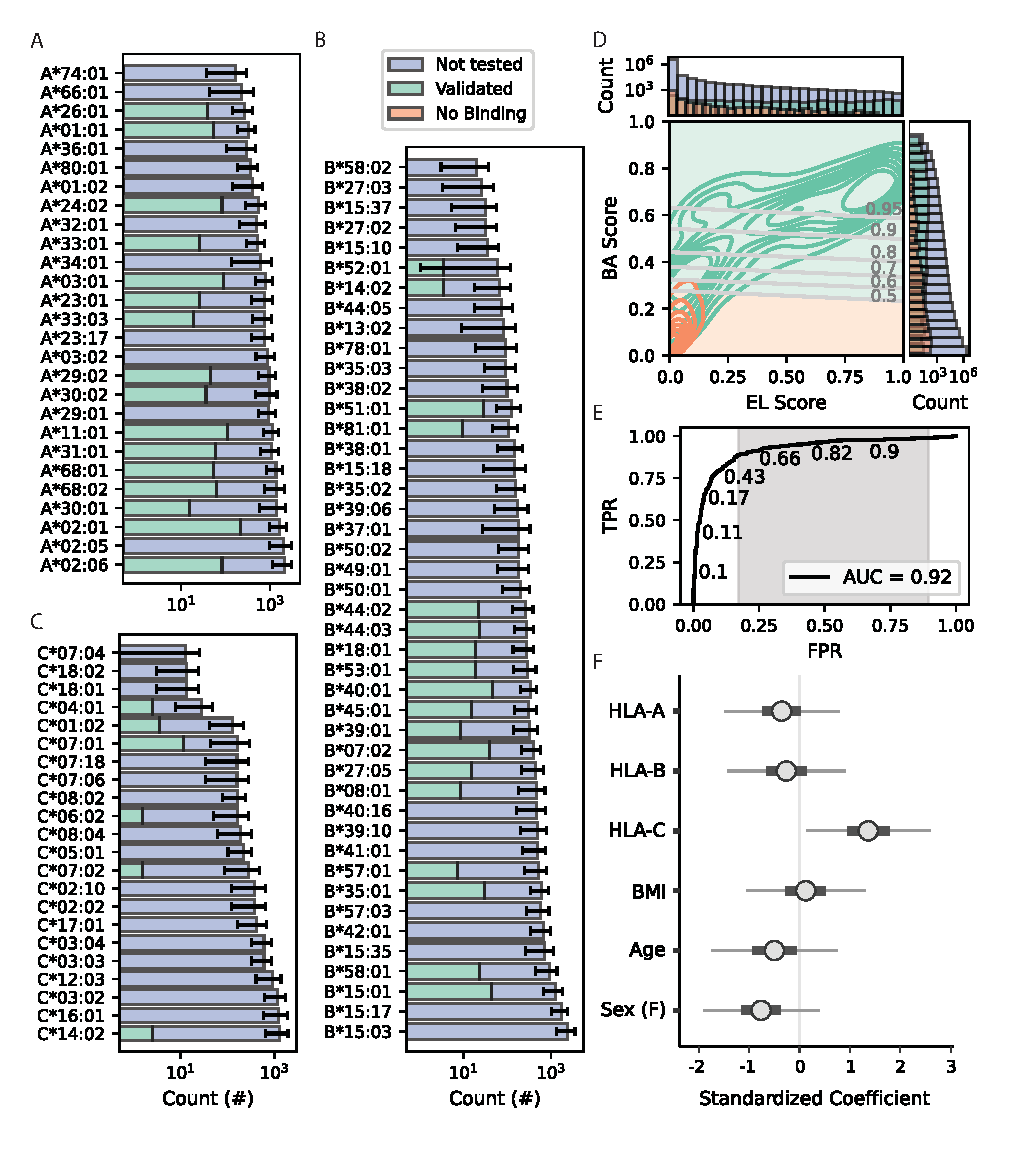
\includegraphics[width=10cm]{Figure1}% This is a *.eps file
\end{center}
\caption{Infection severity correlates with total numbers of predicted HLA-C/SARS-CoV-2 peptide interactions. (A-C) Total numbers of SARS-CoV-2 peptides predicted to bind each MHC molecule (purple bars). Error bars represent standard deviation across probability thresholds. Subsets of interactions documented in the IEDB are shown as green bars. (D) Contour plot and bar plots showing distributions of netMHCpan BA and EL scores for predicted interactions. Green and orange lines/bars correspond to interactions showing positive and negative binding in the IEDB, respectively. Purple bars show the total numbers of predicted binding interactions. Gray lines indicate probability thresholds for positive binding. (E) ROC analysis of logistic regression probability model for identifying positive binding predictions. (F) Forest plot showing standardized multiple linear regression coefficients (circles) for predictors of patient SOFA scores, including 50\% (thick lines) and 95\% (thin lines) confidence intervals.}\label{fig:1}
\end{figure}

\begin{figure}[h!]
\begin{center}
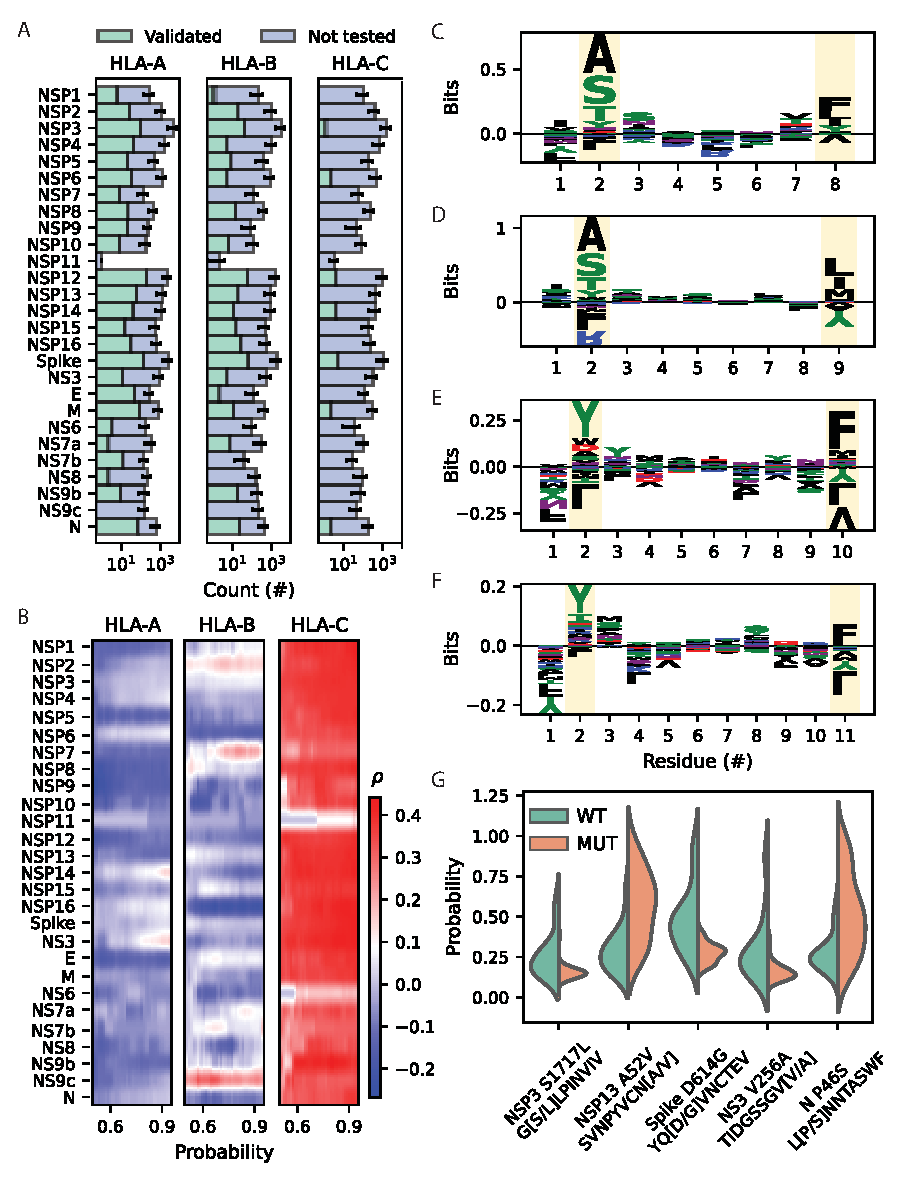
\includegraphics[width=10cm]{Figure2}% This is a *.eps file
\end{center}
\caption{Severity of illness correlates with predicted HLA-C-mediated recognition of both structural and non-structural SARS-CoV-2 protein sequences. (A) Distribution of predicted MHC class I binding across the SARS-CoV-2 proteome. (B) Heatmaps showing correlation between predicted numbers of binding interactions and SOFA score accross SARS-CoV-2 proteins. (C-F) Sequence enrichment plots for 8 to 11 aa peptides exhibiting greatest magnitude correlation (top 1\%) between HLA-C binding probability and SOFA score. (G) Split violin plots showing effects of missense mutations on predicted binding probability toward patient HLA-C molecules. Binding probability distributions for wild-type (Wuhan strain) and mutant strains are shown in green on the left and orange on the right, respectively. All distributions shown are significantly different between wild-type and mutant peptides (p$<$0.05).}\label{fig:2}
\end{figure}

\begin{figure}[h!]
\begin{center}
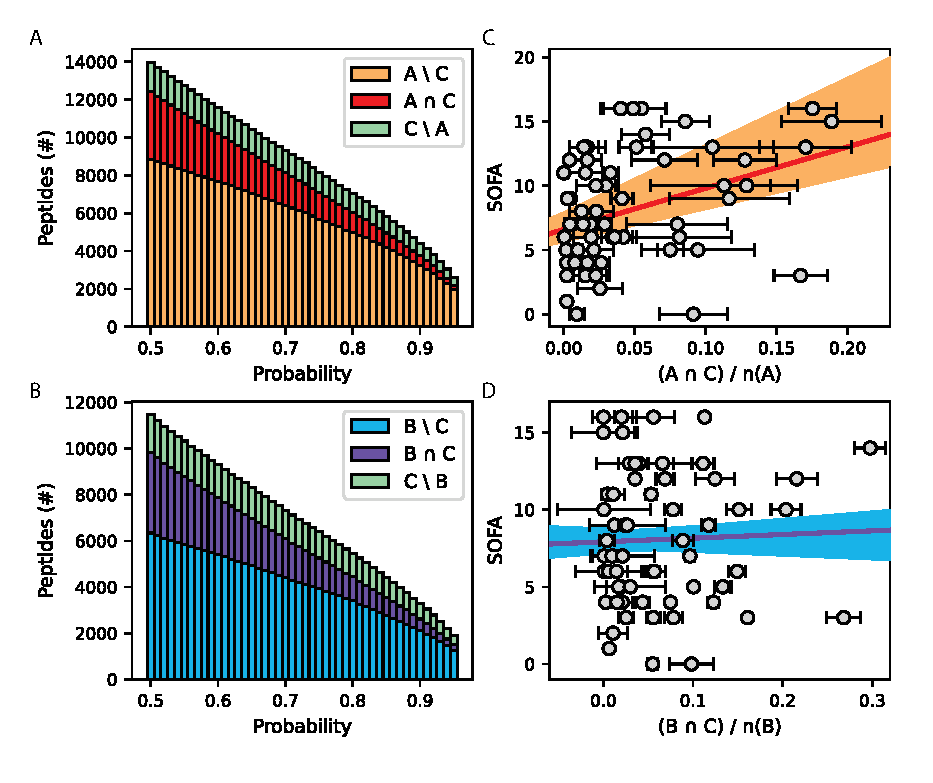
\includegraphics[width=10cm]{Figure3}% This is a *.eps file
\end{center}
\caption{Infection severity correlates with extent of overlap between SARS-CoV-2 peptide repertoires for patient HLA-A and -C molecules. (A-B) Stacked bar chart showing the intersection and differences between sets of SARS-CoV-2 peptides predicted to bind patient HLA-A, -B and -C molecules. (C-D) Results of linear regression using fractional intersection of peptide sets predicted to bind patient HLA-A/B and -C molecules to predict SOFA score. Error bars represent standard deviation across probability thresholds}\label{fig:3}
\end{figure}

\begin{figure}[h!]
\begin{center}
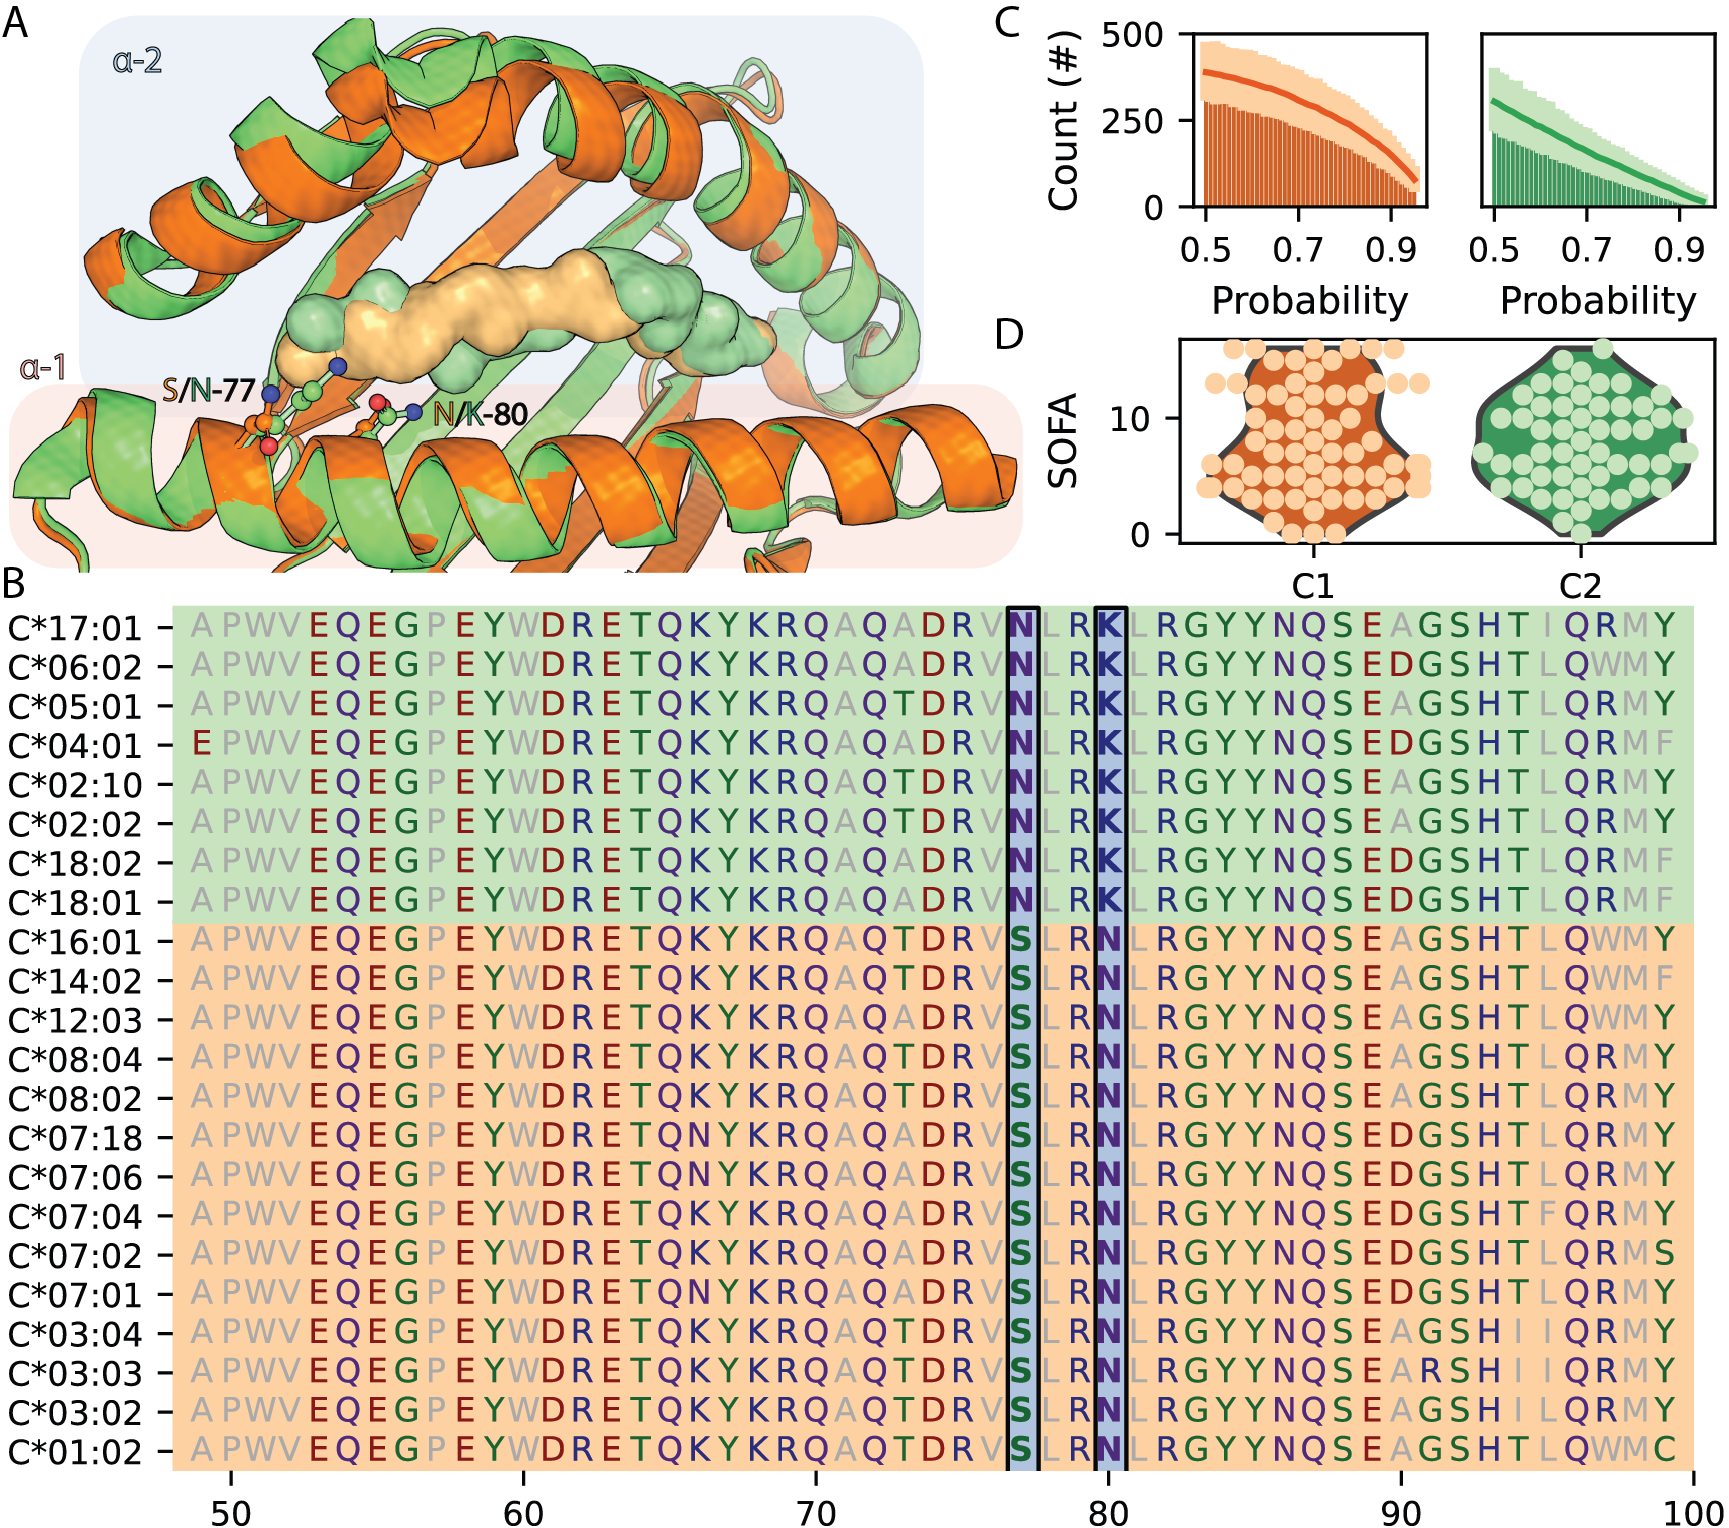
\includegraphics[width=10cm]{Figure4}% This is a *.eps file
\end{center}
\caption{Relationship between KIR cluster, predicted SARS-CoV-2 peptide binding, and illness severity. (A) Structural overlay of C1 (HLA-C*06:02; PDB ID 5W6A) and C2 (HLA-C*07:02; 5VGE) molecules. (B) Protein Sequence alignment of HLA-C $\alpha$-1 helices. (C) Mean numbers of predicted SARS-CoV-2 peptide binding interactions for C1 and C2 molecules as a function of probability threshold. (D) Distributions of patient SOFA scores corresponding to C1 and C2 alleles.}\label{fig:4}
\end{figure}

\begin{figure}[h!]
\begin{center}
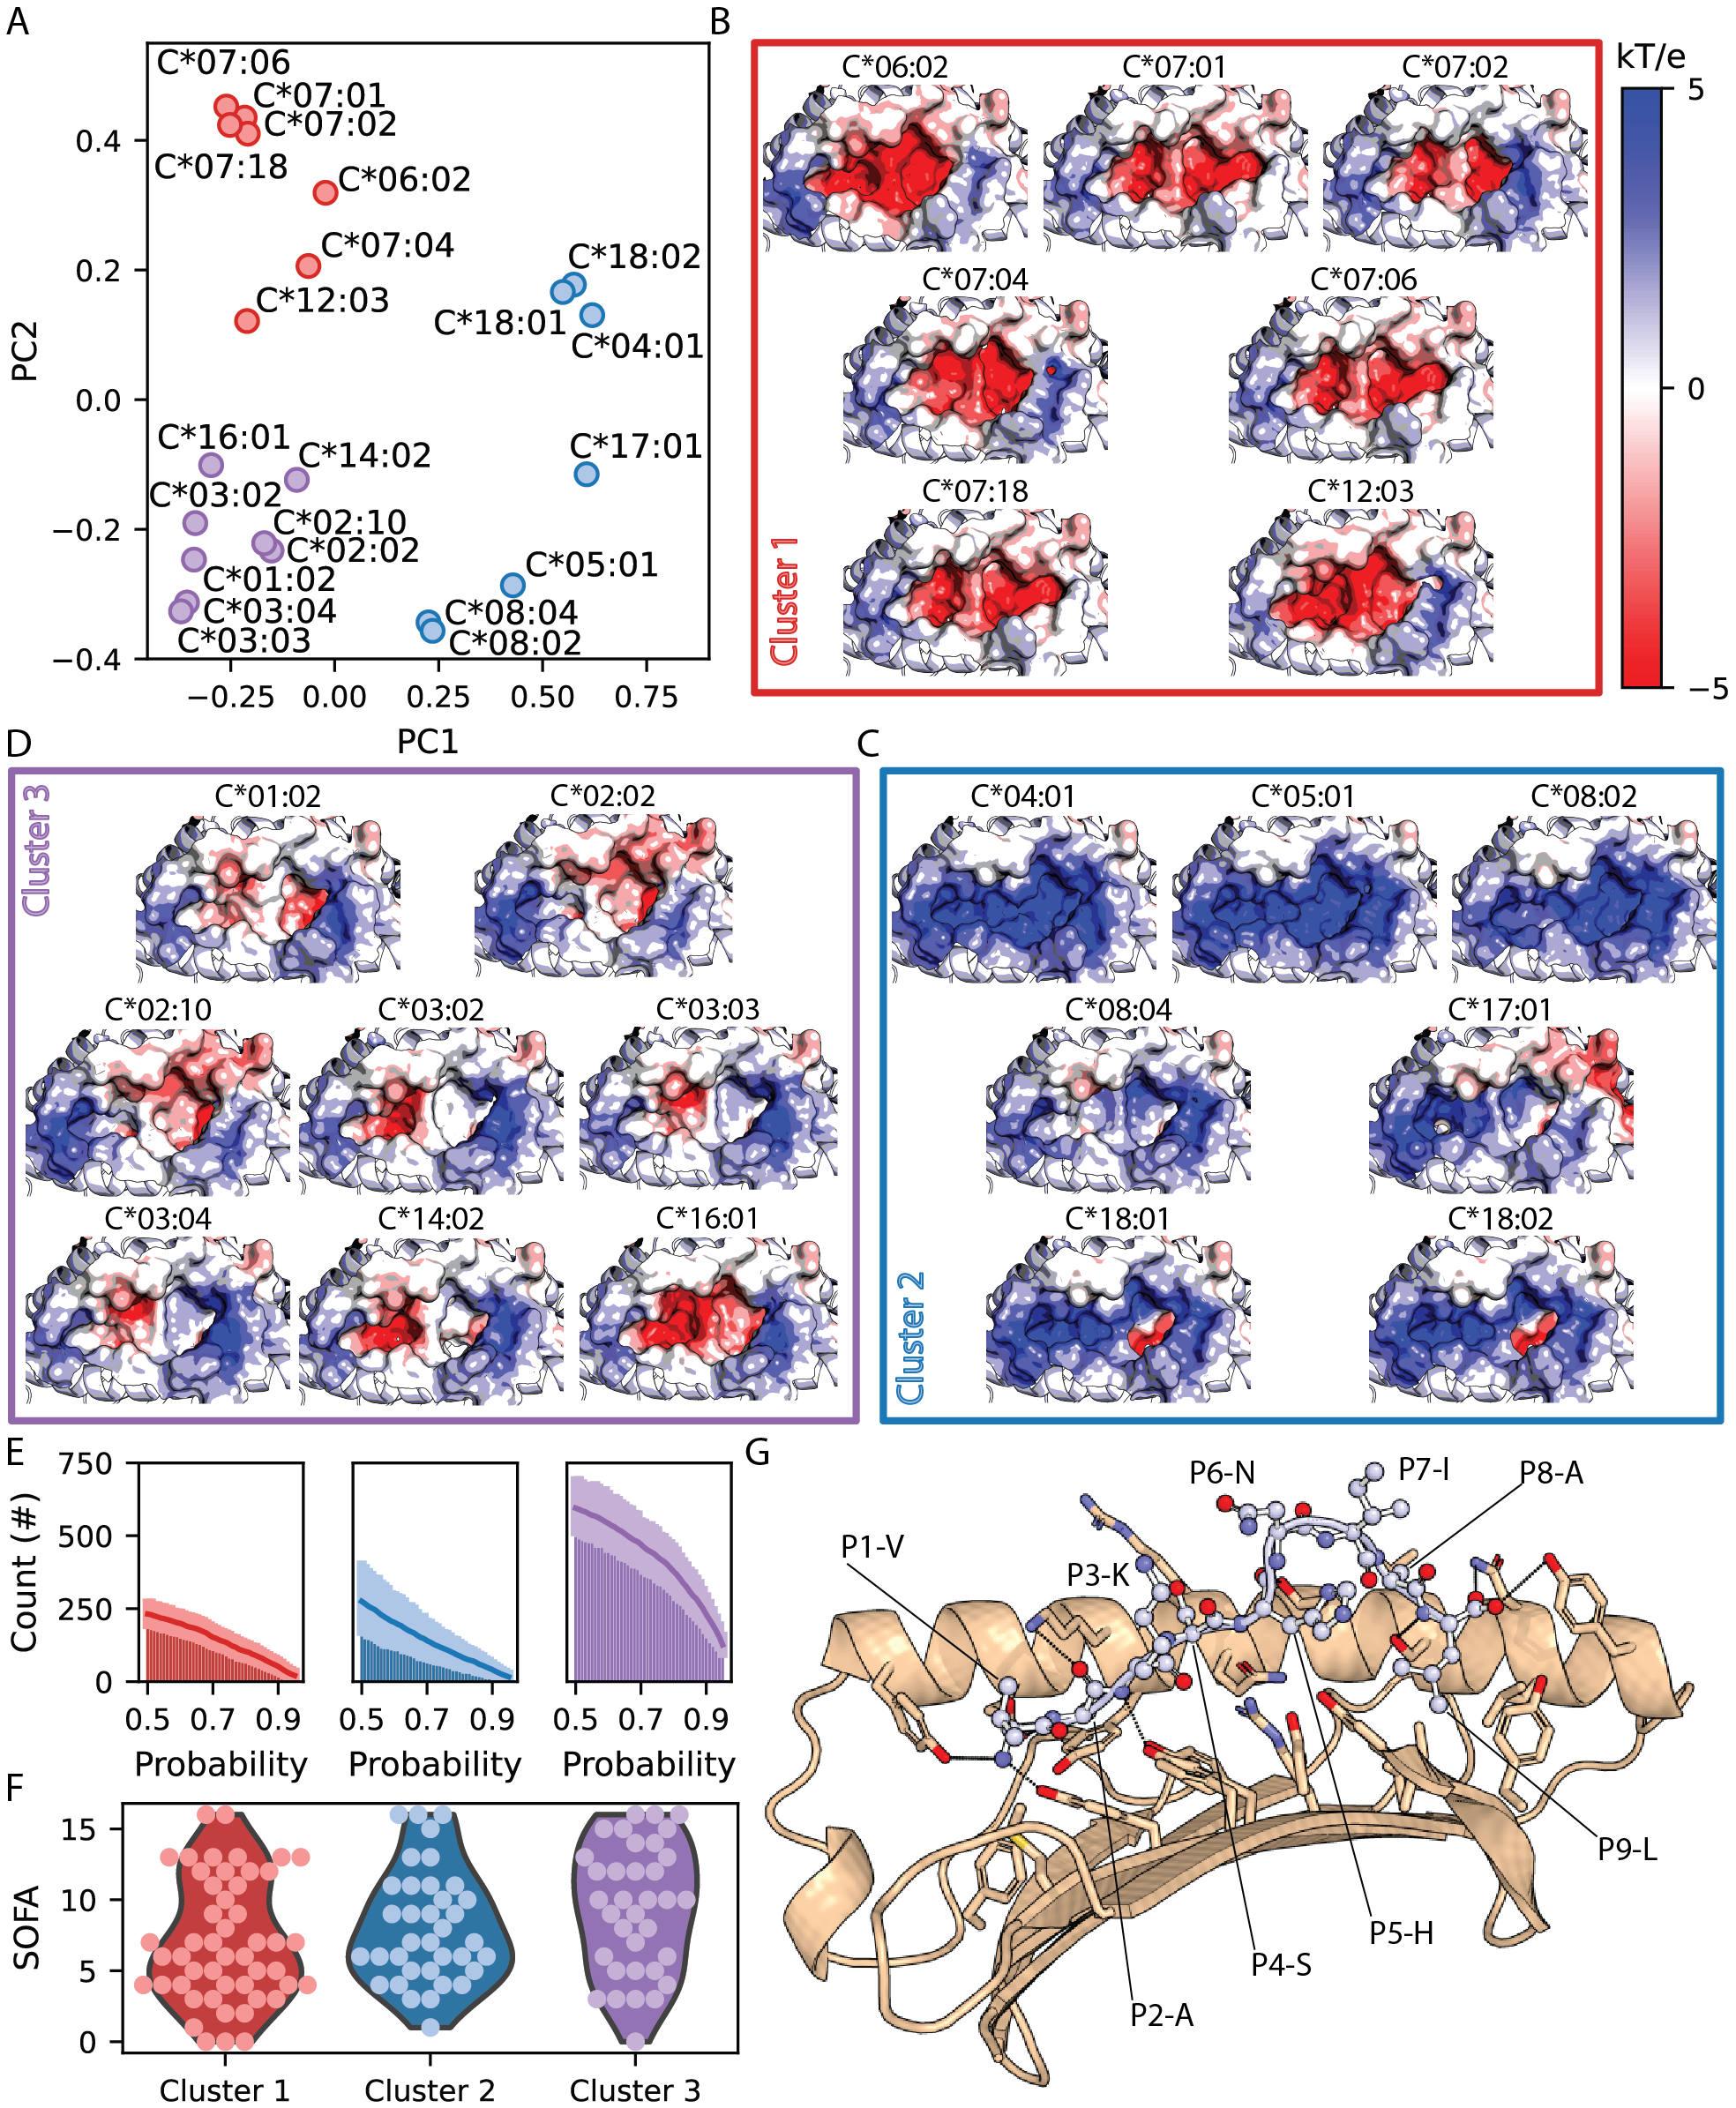
\includegraphics[width=10cm]{Figure5}% This is a *.eps file
\end{center}
\caption{Effect of HLA-C peptide binding surface amino acid composition on predicted peptide repertoire and infection severity. (A) PCA and K-means clustering of patient HLA-C amino acid sequences. (B-D) Electrostatic surface maps of HLA-C peptide binding pockets grouped by sequence-based cluster. (E) Mean numbers of predicted SARS-CoV-2 peptide binding interactions for each cluster across probability threshold. (F) Distribution of patient SOFA scores for alleles in each cluster. (G) Docked structure of HLA-C*03:04 bound to a 9 amino-acid SARS-CoV-2 NSP3 peptide (residues 1885-1894, UniProt ID: P0DTC1).}\label{fig:5}
\end{figure}

\end{document}
